\chapter{Introdução} \label{cap:cap1}

Nas anestesias raquidianas os anestesistas dependem do seu sentimento tátil durante a inserção da agulha no paciente para a correta identificação do local de aplicação do líquido anestésico. O local de aplicação da raquidiana é conhecidos como espaço subaracnóideo \cite{Miller2009}). Para que o anestesista reconheça a chegada da agulha neste local ele precisa reconhecer os tecidos ultrapassados por ela. As anestesias possuem técnicas específicas para identificação dos seus espaços de aplicação. Para que os médicos dominem a técnica da anestesia raquidiana é estimado que são necessários 44 ± 6 repetições de execução deste tipo de procedimento. A confirmação de que o local adequado foi atingido na anestesia raquidiana é feita através da observação do vazamento, através da agulha de punção, do liquido cérebro espinhal ou cefalorraquidiano (\textit{líquor}). As Figuras~\ref{fig:puncaoLombar} e ~\ref{fig:gotejamentoLiquor}  ilustram dois momentos importantes da anestesia raquidiana retirados de um video. Na Figura~\ref{fig:puncaoLombar} é mostrado o momento de inserção da agulha para punção lombar e na Figura~\ref{fig:gotejamentoLiquor} é mostrado o vazamento, através da agulha de punção, do (\textit{líquor}), o que acontece alguns segundos após a agulha estar corretamente posicionada no espaço subaracnóideo. Neste tipo de anestesia é usada uma agulha de menor diâmetro do que a agulha utilizada na anestesia epidural \cite{Miller2009}. O ultrassom é uma ferramenta eficiente para auxilio na determinação do espaço onde a agulha precisa ser inserida \cite{Helayel2010}, mas o uso deste tipo de equipamento não é uma realidade em muitos centros do Brasil \cite{Hamaji2016}. O uso deste equipamento, portanto não faz parte do treinamento de muitas faculdades de medicina para anestesias raquidianas. Este treinamento é feito através da palpação da crista ilíaca do paciente. 

\begin{figure}[h!]
    \centering
    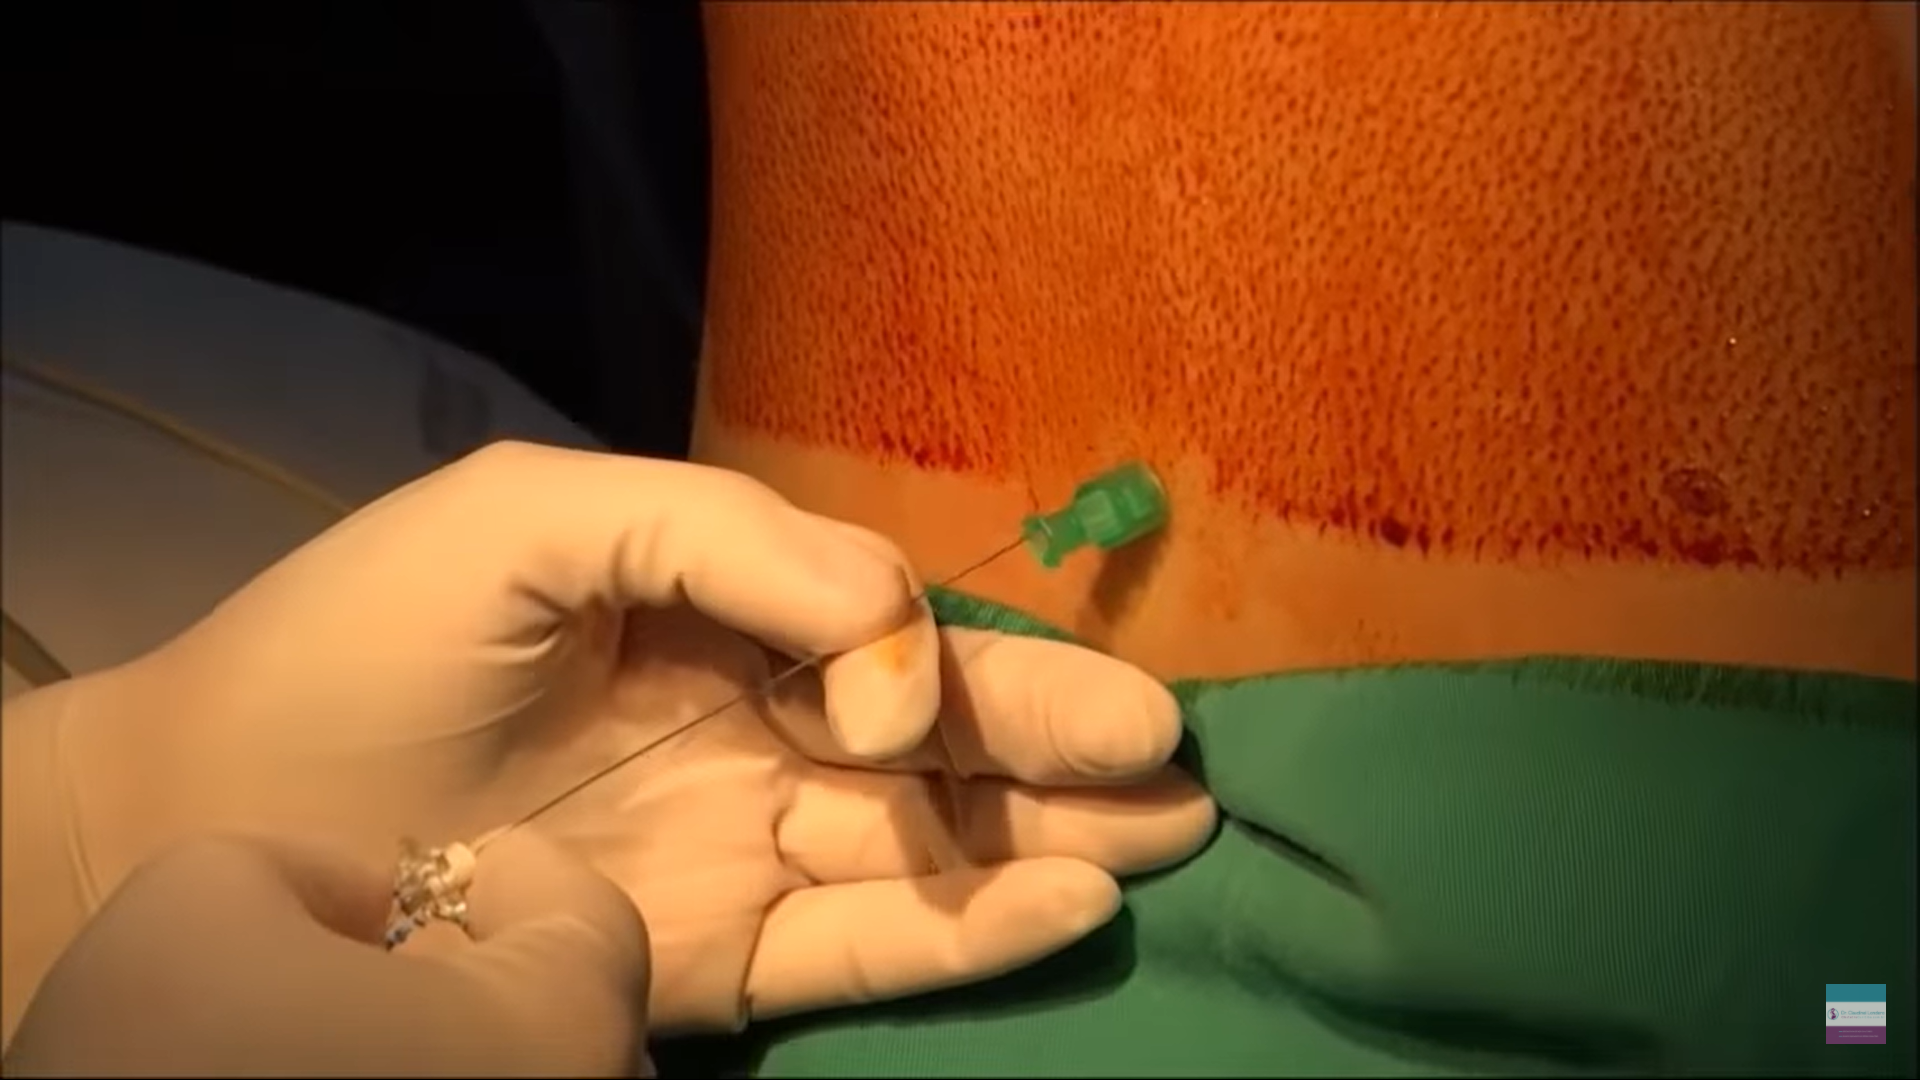
\includegraphics[scale=0.35,keepaspectratio=true]{figuras/2.PuncaoLombar.png} 
    \caption{Punção lombar com agulha de raquianestesia  \cite{Londero2018}.}
    \label{fig:puncaoLombar}
\end{figure}

\begin{figure}[h!]
    \centering
    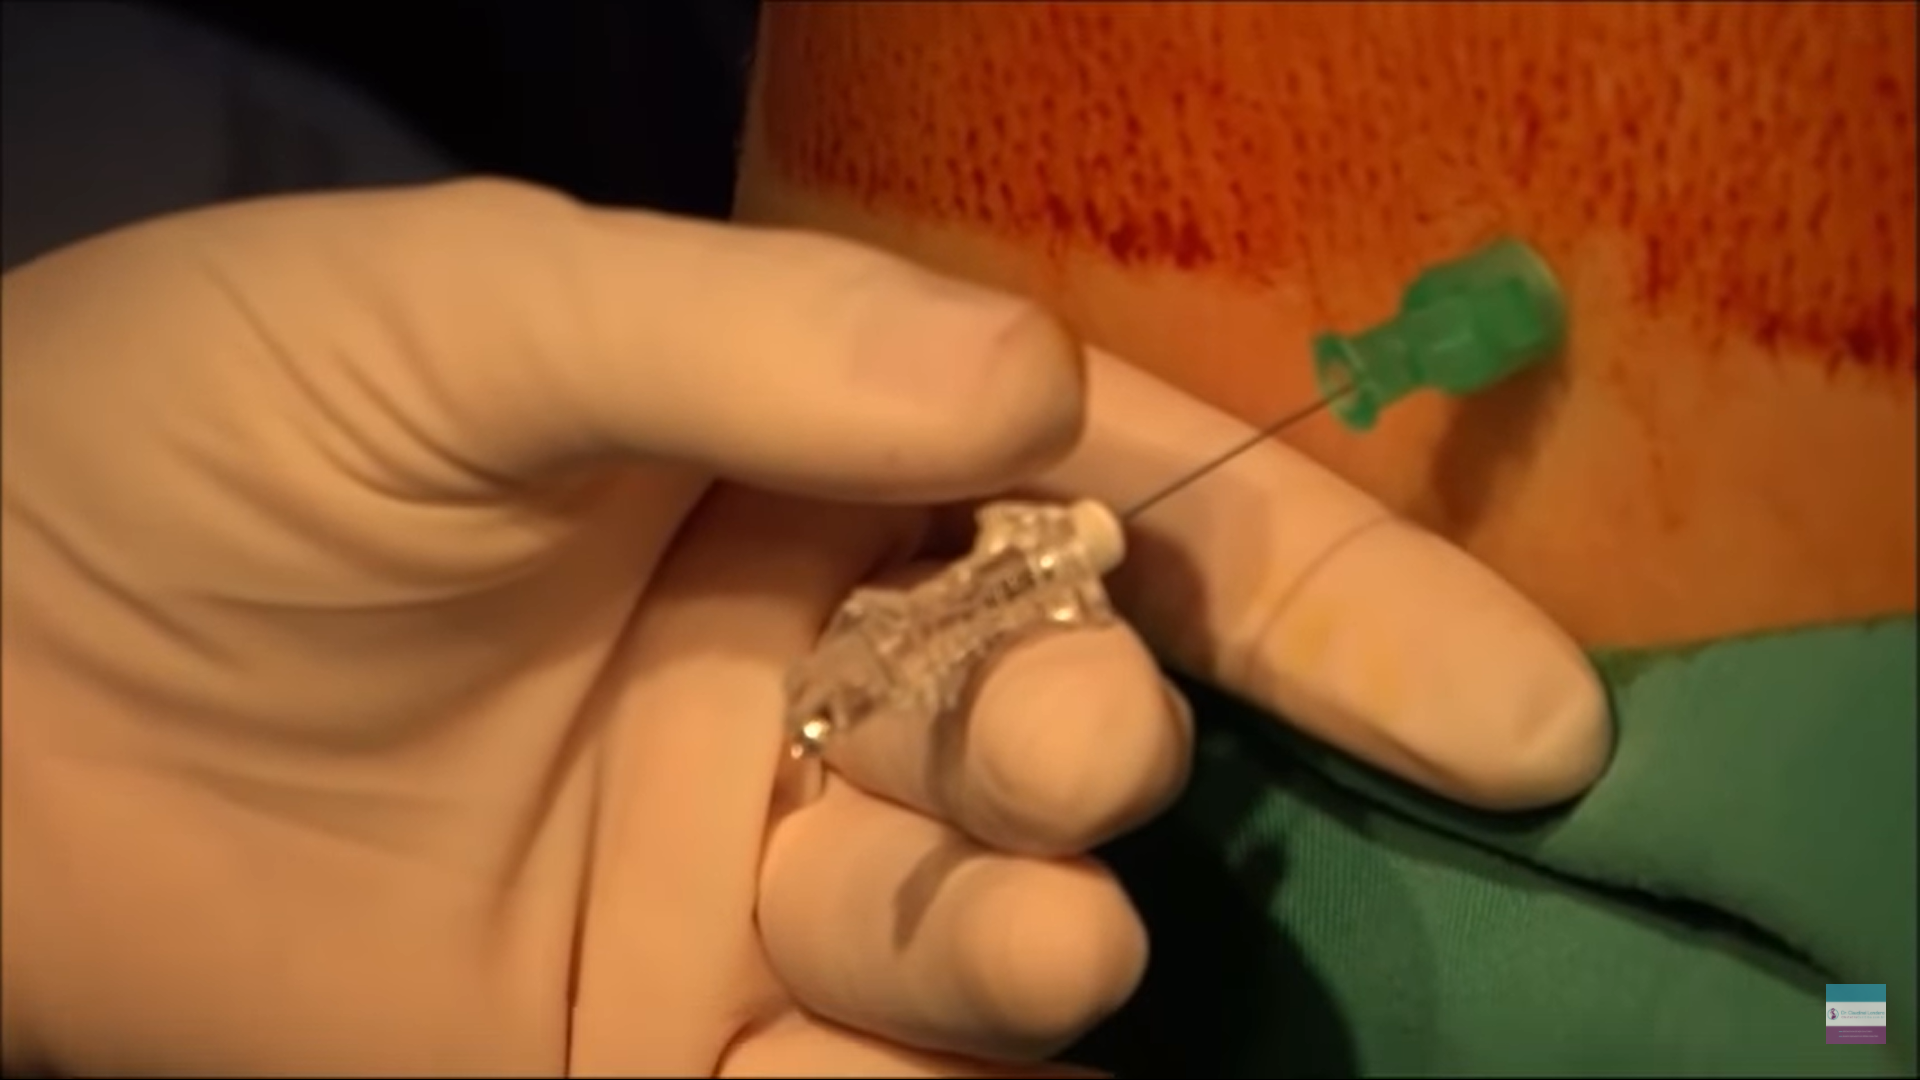
\includegraphics[scale=0.35,keepaspectratio=true]{figuras/3.GotejamentoLiquor.png}
    \caption{Gotejamento do \textit{líquor}, indicação do local correto para a raquianestesia \cite{Londero2018}.}
    \label{fig:gotejamentoLiquor}
\end{figure}

A principal abordagem de treinamento para técnicas de anestesia envolve a observação da aplicação das técnicas por anestesistas experientes. Estes orientam verbalmente os aprendizes conforme cada um dos passos é executado. Adicionalmente a isto são usados: desenhos 2D, cadáveres para demonstração do procedimento, apresentação de vídeos de procedimentos, visualização 3D e técnicas de simulação. No que diz respeito ao treinamento das sensações táteis além do treinamento em cadáveres alguns simuladores fazem uso de bonecos com tecidos artificiais \textit{phantoms} que simulam pacientes \cite{Dreifaldt2006}. Um ponto negativo importante no uso de \textit{phantoms} e de cadáveres, talvez o principal, é a baixa representatividade no que diz respeito a reprodução da situação real, pois estes oferecem uma baixa variabilidade de cenários (pacientes) para treinamento.  Outro aspecto relevante no uso de \textit{phantoms} é a necessidade de reposição de peças que se desgastam com o uso e podem ter custos altos. Estes são alguns dos motivos para que em diversos hospitais a primeira experiência do anestesista em treinamento seja efetuada diretamente em um paciente \cite{Aggarwal2009, Grantcharov2008, Smith2005, Watterson2007}. Esta prática, apesar de ser efetuada sob supervisão direta, traz riscos para estes pacientes e possíveis inseguranças aos aprendizes. 

O uso de simuladores para adquirir certo grau de habilidade antes de iniciar o procedimento em pacientes minimiza os riscos tanto para o aprendiz quanto para o paciente. O uso de simuladores com diversos cenários padroniza o ensino e possibilita ao aprendiz ter experiência com situações mais variadas.  Esta variabilidade de cenários dificilmente aconteceria na vida real em centros onde o ensino é feito diretamente em pacientes \cite{Udani2015}. Diversos simuladores utilizam dispositivos de força háptica (\textit{force feedback}) para auxiliar o aprendiz a experimentar fisicamente as sensações de resistência modeladas para os tecidos ao praticar procedimentos médicos. Este tipo de abordagem é usada em procedimentos médicos de um modo geral \cite{Escobar-Castillejos2016} assim como no caso mais específico dos procedimentos de anestesia \cite{Vaughan2013}. Existem inúmeras outras formas de como o uso de ferramentas computacionais podem auxiliar no campo da anestesia. Um exemplo é no controle automatizado de quanto anestésico aplicar a partir de respostas de medições dos níveis de consciência do paciente \cite{Mendez2009}.

\section{Ideia Central}


\section{Objetivos}
\label{sec:objetivos}



\section{Contribuições da Tese}
\label{sec:contribuicoes}



\section{Estrutura da Tese}
\label{sec:estrutura}

O restante do texto está estruturado da seguinte forma. O Capítulo~\ref{cap:cap2} comenta os principais conceitos e tecnologias envolvidas no desenvolvimento do ambiente de treinamento proposto.

O Capítulo~\ref{cap:cap3} contém os trabalhos relacionados a esta tese assim como o posicionamento deste trabalho frente aos demais.

No Capítulo~\ref{cap:cap4} é apresentada a proposta de desenvolvimento que foi desenvolvida durantes este trabalho. 

O Capítulo~\ref{cap:cap5} apresenta os experimentos que foram feitos. 

O Capítulo~\ref{cap:cap6} apresenta uma avaliação dos experimentos em relação aos seus resultados.

Por fim, o Capítulo~\ref{cap:cap7} conclui o trabalho, apresentando as conclusões, realçando as contribuições desta tese e apontando os  trabalhos futuros.